
\begin{figure}[h]
	\centering
	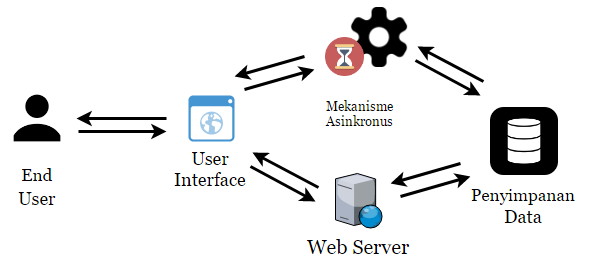
\includegraphics
	[width=\textwidth]
	{images/bab3/buku/basic_architecture.png}
	\caption{Arsitektur Dasar Aplikasi}
	\label{fundamental-component}
\end{figure}

\subsection{Identifikasi Komponen Fundamental}
	Berdasarkan Bab Analisa, dapat diidentifikasi dan divisualisasikan pada Gambar \ref{fundamental-component} yaitu komponen-komponen penting dalam pembuatan aplikasi sebagai berikut:
	\begin{enumerate}
		\item \textit{Webserver}
		\item Mekanisme penyimpanan data (\textit{database} dan \textit{data storage})
		\item \textit{User Interface} sebagai media terhadap \textit{end-user}
		\item Mekanisme Asinkronus untuk mengakomodasi fitur \textit{realtime}
	\end{enumerate}
	
	
	
